\documentclass[varwidth]{standalone}
\usepackage{tikz}
\usepackage{tikz,tcolorbox, tikz-cd}
%\usetikzlibrary{...}
\begin{document}
% \begin{center}
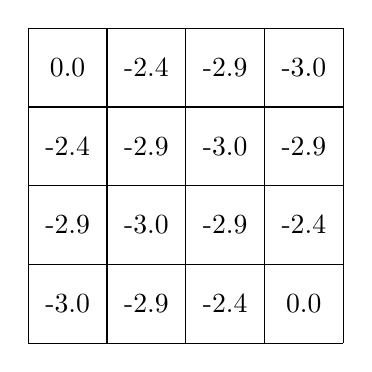
\begin{tikzpicture} 
\begin{scope}[local bounding box=L]
 \fill[black!0] (0,3) rectangle ++ (1,1); 
 \fill[black!0] (3,0) rectangle ++ (1,1); 
 \draw (0,0) grid (4,4); 

 \node at (0.5,3.5) {0.0};
 \node at (1.5,3.5) {-2.4};
 \node at (2.5,3.5) {-2.9};
 \node at (3.5,3.5) {-3.0};

 \node at (0.5,2.5) {-2.4};
 \node at (1.5,2.5) {-2.9};
 \node at (2.5,2.5) {-3.0};
 \node at (3.5,2.5) {-2.9};
 
 \node at (0.5,1.5) {-2.9};
 \node at (1.5,1.5) {-3.0};
 \node at (2.5,1.5) {-2.9};
 \node at (3.5,1.5) {-2.4};
 
 \node at (0.5,0.5) {-3.0};
 \node at (1.5,0.5) {-2.9};
 \node at (2.5,0.5) {-2.4};
 \node at (3.5,0.5) {0.0};

\end{scope} 
\end{tikzpicture} 
\hspace{1cm}
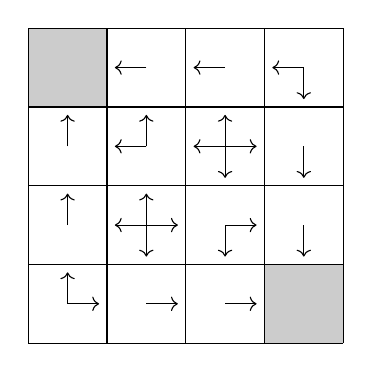
\begin{tikzpicture} 
\begin{scope}[local bounding box=L]
 \fill[black!20] (0,3) rectangle ++ (1,1); 
 \fill[black!20] (3,0) rectangle ++ (1,1); 
 \draw (0,0) grid (4,4); 

 % \node at (1.75,+3.75) {1};
 \draw[->] (1.5,3.5) -- (1.1,3.5);
 % \node at (2.75,+3.75) {2};
 \draw[->] (2.5,3.5) -- (2.1,3.5);
 % \node at (3.75,+3.75) {3};
 \draw[->] (3.5,3.5) -- (3.1,3.5);
 \draw[->] (3.5,3.5) -- (3.5,3.1);
 % \node at (0.75,+2.75) {4};
 \draw[->] (0.5,2.5) -- (0.5,2.9);
 % \node at (1.75,+2.75) {5};
 \draw[->] (1.5,2.5) -- (1.5,2.9);
 \draw[->] (1.5,2.5) -- (1.1,2.5);
 % \node at (2.75,+2.75) {6};
 \draw[->] (2.5,2.5) -- (2.5,2.9);
 \draw[->] (2.5,2.5) -- (2.5,2.1);
 \draw[->] (2.5,2.5) -- (2.9,2.5);
 \draw[->] (2.5,2.5) -- (2.1,2.5);
 % \node at (3.75,+2.75) {7};
 \draw[->] (3.5,2.5) -- (3.5,2.1);
 % \node at (0.75,+1.75) {8};
 \draw[->] (0.5,1.5) -- (0.5,1.9);
 % \node at (1.75,+1.75) {9};
 \draw[->] (1.5,1.5) -- (1.9,1.5);
 \draw[->] (1.5,1.5) -- (1.1,1.5);
 \draw[->] (1.5,1.5) -- (1.5,1.9);
 \draw[->] (1.5,1.5) -- (1.5,1.1);
 % \node at (2.75,+1.75) {10};
 \draw[->] (2.5,1.5) -- (2.9,1.5);
 \draw[->] (2.5,1.5) -- (2.5,1.1);
 % \node at (3.75,+1.75) {11};
 \draw[->] (3.5,1.5) -- (3.5,1.1);
  % \node at (0.75,+0.75) {12};
 \draw[->] (0.5,0.5) -- (0.9,0.5);
 \draw[->] (0.5,0.5) -- (0.5,0.9);
 % \node at (1.75,+0.75) {13};
 \draw[->] (1.5,0.5) -- (1.9,0.5);
 % \node at (2.75,+0.75) {14};
 \draw[->] (2.5,0.5) -- (2.9,0.5);
\end{scope} 
\end{tikzpicture} 


\vspace{1cm}
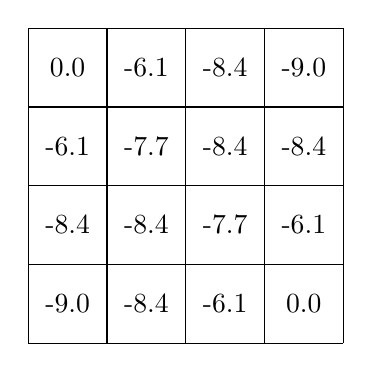
\begin{tikzpicture} 
\begin{scope}[local bounding box=L]
 \fill[black!0] (0,3) rectangle ++ (1,1); 
 \fill[black!0] (3,0) rectangle ++ (1,1); 
 \draw (0,0) grid (4,4); 

 \node at (0.5,3.5) {0.0};
 \node at (1.5,3.5) {-6.1};
 \node at (2.5,3.5) {-8.4};
 \node at (3.5,3.5) {-9.0};

 \node at (0.5,2.5) {-6.1};
 \node at (1.5,2.5) {-7.7};
 \node at (2.5,2.5) {-8.4};
 \node at (3.5,2.5) {-8.4};
 
 \node at (0.5,1.5) {-8.4};
 \node at (1.5,1.5) {-8.4};
 \node at (2.5,1.5) {-7.7};
 \node at (3.5,1.5) {-6.1};
 
 \node at (0.5,0.5) {-9.0};
 \node at (1.5,0.5) {-8.4};
 \node at (2.5,0.5) {-6.1};
 \node at (3.5,0.5) {0.0};

\end{scope} 
\end{tikzpicture} 
\hspace{1cm}
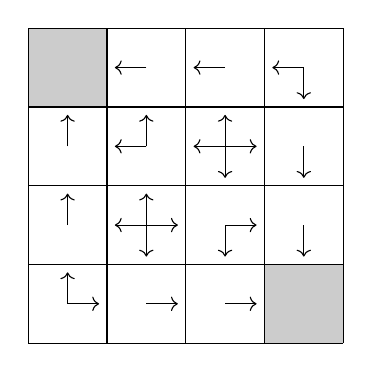
\begin{tikzpicture} 
\begin{scope}[local bounding box=L]
 \fill[black!20] (0,3) rectangle ++ (1,1); 
 \fill[black!20] (3,0) rectangle ++ (1,1); 
 \draw (0,0) grid (4,4); 

 % \node at (1.75,+3.75) {1};
 \draw[->] (1.5,3.5) -- (1.1,3.5);
 % \node at (2.75,+3.75) {2};
 \draw[->] (2.5,3.5) -- (2.1,3.5);
 % \node at (3.75,+3.75) {3};
 \draw[->] (3.5,3.5) -- (3.1,3.5);
 \draw[->] (3.5,3.5) -- (3.5,3.1);
 % \node at (0.75,+2.75) {4};
 \draw[->] (0.5,2.5) -- (0.5,2.9);
 % \node at (1.75,+2.75) {5};
 \draw[->] (1.5,2.5) -- (1.5,2.9);
 \draw[->] (1.5,2.5) -- (1.1,2.5);
 % \node at (2.75,+2.75) {6};
 \draw[->] (2.5,2.5) -- (2.5,2.9);
 \draw[->] (2.5,2.5) -- (2.5,2.1);
 \draw[->] (2.5,2.5) -- (2.9,2.5);
 \draw[->] (2.5,2.5) -- (2.1,2.5);
 % \node at (3.75,+2.75) {7};
 \draw[->] (3.5,2.5) -- (3.5,2.1);
 % \node at (0.75,+1.75) {8};
 \draw[->] (0.5,1.5) -- (0.5,1.9);
 % \node at (1.75,+1.75) {9};
 \draw[->] (1.5,1.5) -- (1.9,1.5);
 \draw[->] (1.5,1.5) -- (1.1,1.5);
 \draw[->] (1.5,1.5) -- (1.5,1.9);
 \draw[->] (1.5,1.5) -- (1.5,1.1);
 % \node at (2.75,+1.75) {10};
 \draw[->] (2.5,1.5) -- (2.9,1.5);
 \draw[->] (2.5,1.5) -- (2.5,1.1);
 % \node at (3.75,+1.75) {11};
 \draw[->] (3.5,1.5) -- (3.5,1.1);
  % \node at (0.75,+0.75) {12};
 \draw[->] (0.5,0.5) -- (0.9,0.5);
 \draw[->] (0.5,0.5) -- (0.5,0.9);
 % \node at (1.75,+0.75) {13};
 \draw[->] (1.5,0.5) -- (1.9,0.5);
 % \node at (2.75,+0.75) {14};
 \draw[->] (2.5,0.5) -- (2.9,0.5);
\end{scope} 
\end{tikzpicture} 

\vspace{1cm}
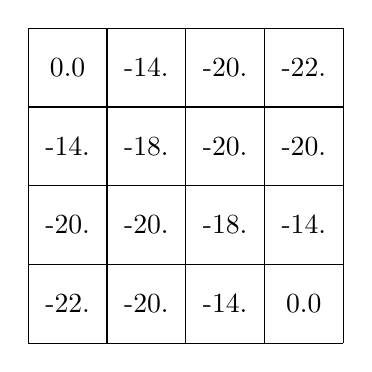
\begin{tikzpicture} 
\begin{scope}[local bounding box=L]
 \fill[black!0] (0,3) rectangle ++ (1,1); 
 \fill[black!0] (3,0) rectangle ++ (1,1); 
 \draw (0,0) grid (4,4); 

 \node at (0.5,3.5) {0.0};
 \node at (1.5,3.5) {-14.};
 \node at (2.5,3.5) {-20.};
 \node at (3.5,3.5) {-22.};

 \node at (0.5,2.5) {-14.};
 \node at (1.5,2.5) {-18.};
 \node at (2.5,2.5) {-20.};
 \node at (3.5,2.5) {-20.};
 
 \node at (0.5,1.5) {-20.};
 \node at (1.5,1.5) {-20.};
 \node at (2.5,1.5) {-18.};
 \node at (3.5,1.5) {-14.};
 
 \node at (0.5,0.5) {-22.};
 \node at (1.5,0.5) {-20.};
 \node at (2.5,0.5) {-14.};
 \node at (3.5,0.5) {0.0};

\end{scope} 
\end{tikzpicture} 
\hspace{1cm}
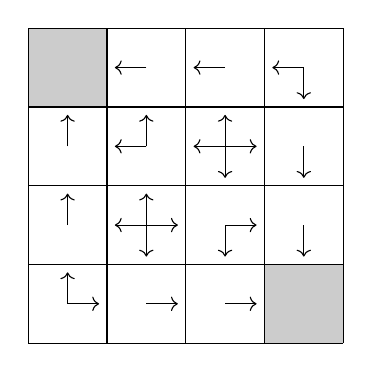
\begin{tikzpicture} 
\begin{scope}[local bounding box=L]
 \fill[black!20] (0,3) rectangle ++ (1,1); 
 \fill[black!20] (3,0) rectangle ++ (1,1); 
 \draw (0,0) grid (4,4); 

 % \node at (1.75,+3.75) {1};
 \draw[->] (1.5,3.5) -- (1.1,3.5);
 % \node at (2.75,+3.75) {2};
 \draw[->] (2.5,3.5) -- (2.1,3.5);
 % \node at (3.75,+3.75) {3};
 \draw[->] (3.5,3.5) -- (3.1,3.5);
 \draw[->] (3.5,3.5) -- (3.5,3.1);
 % \node at (0.75,+2.75) {4};
 \draw[->] (0.5,2.5) -- (0.5,2.9);
 % \node at (1.75,+2.75) {5};
 \draw[->] (1.5,2.5) -- (1.5,2.9);
 \draw[->] (1.5,2.5) -- (1.1,2.5);
 % \node at (2.75,+2.75) {6};
 \draw[->] (2.5,2.5) -- (2.5,2.9);
 \draw[->] (2.5,2.5) -- (2.5,2.1);
 \draw[->] (2.5,2.5) -- (2.9,2.5);
 \draw[->] (2.5,2.5) -- (2.1,2.5);
 % \node at (3.75,+2.75) {7};
 \draw[->] (3.5,2.5) -- (3.5,2.1);
 % \node at (0.75,+1.75) {8};
 \draw[->] (0.5,1.5) -- (0.5,1.9);
 % \node at (1.75,+1.75) {9};
 \draw[->] (1.5,1.5) -- (1.9,1.5);
 \draw[->] (1.5,1.5) -- (1.1,1.5);
 \draw[->] (1.5,1.5) -- (1.5,1.9);
 \draw[->] (1.5,1.5) -- (1.5,1.1);
 % \node at (2.75,+1.75) {10};
 \draw[->] (2.5,1.5) -- (2.9,1.5);
 \draw[->] (2.5,1.5) -- (2.5,1.1);
 % \node at (3.75,+1.75) {11};
 \draw[->] (3.5,1.5) -- (3.5,1.1);
  % \node at (0.75,+0.75) {12};
 \draw[->] (0.5,0.5) -- (0.9,0.5);
 \draw[->] (0.5,0.5) -- (0.5,0.9);
 % \node at (1.75,+0.75) {13};
 \draw[->] (1.5,0.5) -- (1.9,0.5);
 % \node at (2.75,+0.75) {14};
 \draw[->] (2.5,0.5) -- (2.9,0.5);
\end{scope} 
\end{tikzpicture}  
% \end{center}
\end{document}
